\section{Container Escapes}\label{subsection:container-escape}
In a container escape, an attacker has gained access to a container and tries to escape its isolation. When an attacker gains access to a container, they have gained a foothold inside their target, but that foothold is (like everything else inside the container) isolated from the host. Container escapes focus on attacking and bypassing the isolation and protection mechanics that separate the container from the host and other containers.

\medskip

\begin{figure}[ht]
    \centering
    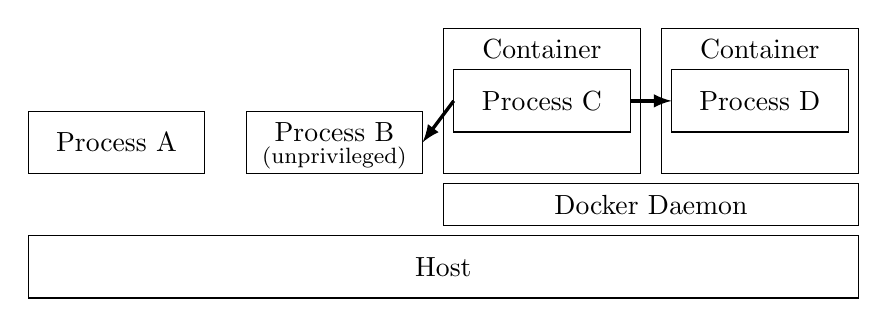
\begin{tikzpicture}[x=0.75pt,y=0.75pt,yscale=-1,xscale=1]
        % Host Rectangle
        \draw (0,100) -- (400,100) -- (400,130) -- (0,130) -- cycle ;
        \draw (200, 115) node {Host};

        %Docker Daemon Rectangle
        \draw (200,75) -- (400,75) -- (400,95) -- (200,95) -- cycle ;
        \draw (300,85) node {Docker Daemon};

        % Process A Rectangle
        \draw (0,40) -- (85,40) -- (85,70) -- (0,70) -- cycle ;
        \draw (42.5,55) node {Process A};

        % Process B Rectangle
        \draw (105,40) -- (190,40) -- (190,70) -- (105,70) -- cycle ;
        \draw (147.5,50) node {Process B};
        \draw (147.5,62.5) node {{\footnotesize (unprivileged)}};

        %Container Process C Rectangle
        \draw (200,0) -- (295,0) -- (295,70) -- (200,70) -- cycle ;
        \draw (247.5,10) node {Container};

        %% Process C Rectangle
        \draw (205,20) -- (290,20) -- (290,50) -- (205,50) -- cycle ;
        \draw (247.5,35) node {Process C};

        %Container Process D Rectangle
        \draw (305,0) -- (400,0) -- (400,70) -- (305,70) -- cycle ;
        \draw (352.5,10) node {Container};

        %% Process D Rectangle
        \draw (310,20) -- (395,20) -- (395,50) -- (310,50) -- cycle ;
        \draw (352.5,35) node {Process D};

        % Lines
        \draw [latex-,very thick] (190,55) -- (205,35) ;
        \draw [-latex, very thick] (290,35) -- (310,35) ;
    \end{tikzpicture}
    \caption{}\label{fig:container-escape}
    \medskip
    \small
    A process (Process C) running inside a container accessing data on the host (that it should not be able to access), in this case Process B.
\end{figure}

In \autoref{fig:container-escape} we see two variants of container escapes. We see Process C accessing Process B, which is a process that runs directly on the host. We also see Process C accessing Process D, which is inside another container. In both cases Process C escapes the isolation of the container and accesses data that it should not have access too.

In the first variant, Process C escapes the container to access data that it should not have access to on the host.

In the second variant, Process C escapes from its container and accesses another container. Containers should not only be isolated from the host, but also from other containers. This allows multiple containers with sensitive data to be run on the same host without them being able to access each other's data.

\medskip

An example attack scenario would be a company that offers Platform as a Service (PaaS) products that allows customers to run Docker containers on their infrastructure.\footnote{This is quite common nowadays. All major computing providers offer such a service.} If it is possible for the attacker to submit a Docker image with a malicious process that escapes the container and access the underlying infrastructure, they could access other containers or other internal resources. That would, obviously, be a big problem for the company.

\medskip

It should be noted that an exploit that allows someone to escape from a Linux \lstinline{namespace} is essentially a container escape exploit, because Docker relies heavily on \lstinline{namespaces} for isolation (see \autoref{subsubsection:internals}). CVE--2017--7308~\cite{CVE-2017-7308} is a good example of this.
